\documentclass{beamer}
\usepackage[latin1]{inputenc}
\usepackage{enumerate}
\usepackage{graphicx}
\usepackage{wrapfig}
\usepackage{amssymb}
\usepackage{epstopdf}
\usepackage{amsthm}
\usepackage{tipa}
\usepackage{color}
\usepackage{wasysym}
\usepackage{setspace}
\usepackage{tcolorbox}

\renewcommand{\baselinestretch}{1.0}
% \usepackage{beamerthemesplit} // Activate for custom appearance

\title{High-dimensional local optimization in variational inference}
\author{Otte Hein�vaara \\
\vspace{1cm}
Antti Honkela \\
Probabilistic Inference and Computational Biology (PROBIC) \\
Statistical Machine Learning and Bioinformatics \\
HIIT}
\date{\today}


\begin{document}

\begin{frame}
\titlepage
\end{frame}


\begin{frame}
\frametitle{Variational inference}
\begin{tabular}{c  c  l}
\textbf{Bayes' rule} &$-$ &$P(Z | E) = \frac{P(Z)}{P(E)}P(E | Z)$\\
$\Downarrow$ \\
\textbf{Bayesian inference}  & $-$ &$ P(Z | E) = \frac{P(Z)}{\sum_{i} P(E | Z_{i})P(Z_{i})}P(E | Z)$\\
$\Downarrow$ \\
\textbf{Variational inference} & $-$ &$P(Z | E) \approx Q(Z)$
\end{tabular}
\end{frame}

\begin{frame}
\frametitle{Topic models}
\noindent

{\Large\bfseries How does a machine discover a topic?}
\vspace{1cm}

\begin{columns}[T] % align columns
\begin{column}{.45\textwidth}
\rule{\linewidth}{1pt}
This study is about the science of food. Do you like pizza or pasta? Is there way to determine how tasty food is without tasting or smelling it?
\end{column}%
\hfill%

\begin{column}{.1\textwidth}\centering
\vspace{1.0cm}
$\hbox{\scalebox{2}{\Huge\pointer}}$
\end{column}%

\begin{column}{.45\textwidth}
\rule{\linewidth}{1pt}
This \textcolor{blue}{study} is about the \textcolor{blue}{science} of \textcolor{orange}{food}. Do you like \textcolor{orange}{pizza} or \textcolor{orange}{pasta}? Is there way to \textcolor{blue}{determine} how \textcolor{orange}{tasty} \textcolor{orange}{food} is without \textcolor{orange}{tasting} or \textcolor{orange}{smelling} it? \\
$$
\text{Words related to}
\left.
\begin{array}{c}
\text{\textcolor{orange}{\textbf{food}}} \\ 
\text{\textcolor{blue}{\textbf{science}}}
\end{array}
\right.
$$

\end{column}%
\end{columns}


\end{frame}



\begin{frame}
\frametitle{LDA - Latent Dirichlet Allocation}
{\setstretch{1.0}\tiny D. M. Blei, A. Y. Ng, and M. I. Jordan. Latent Dirichlet allocation. \textit{The Journal of Machine Learning Research}, 3:993-1022, 2003. \\}
\vspace{0.4cm}
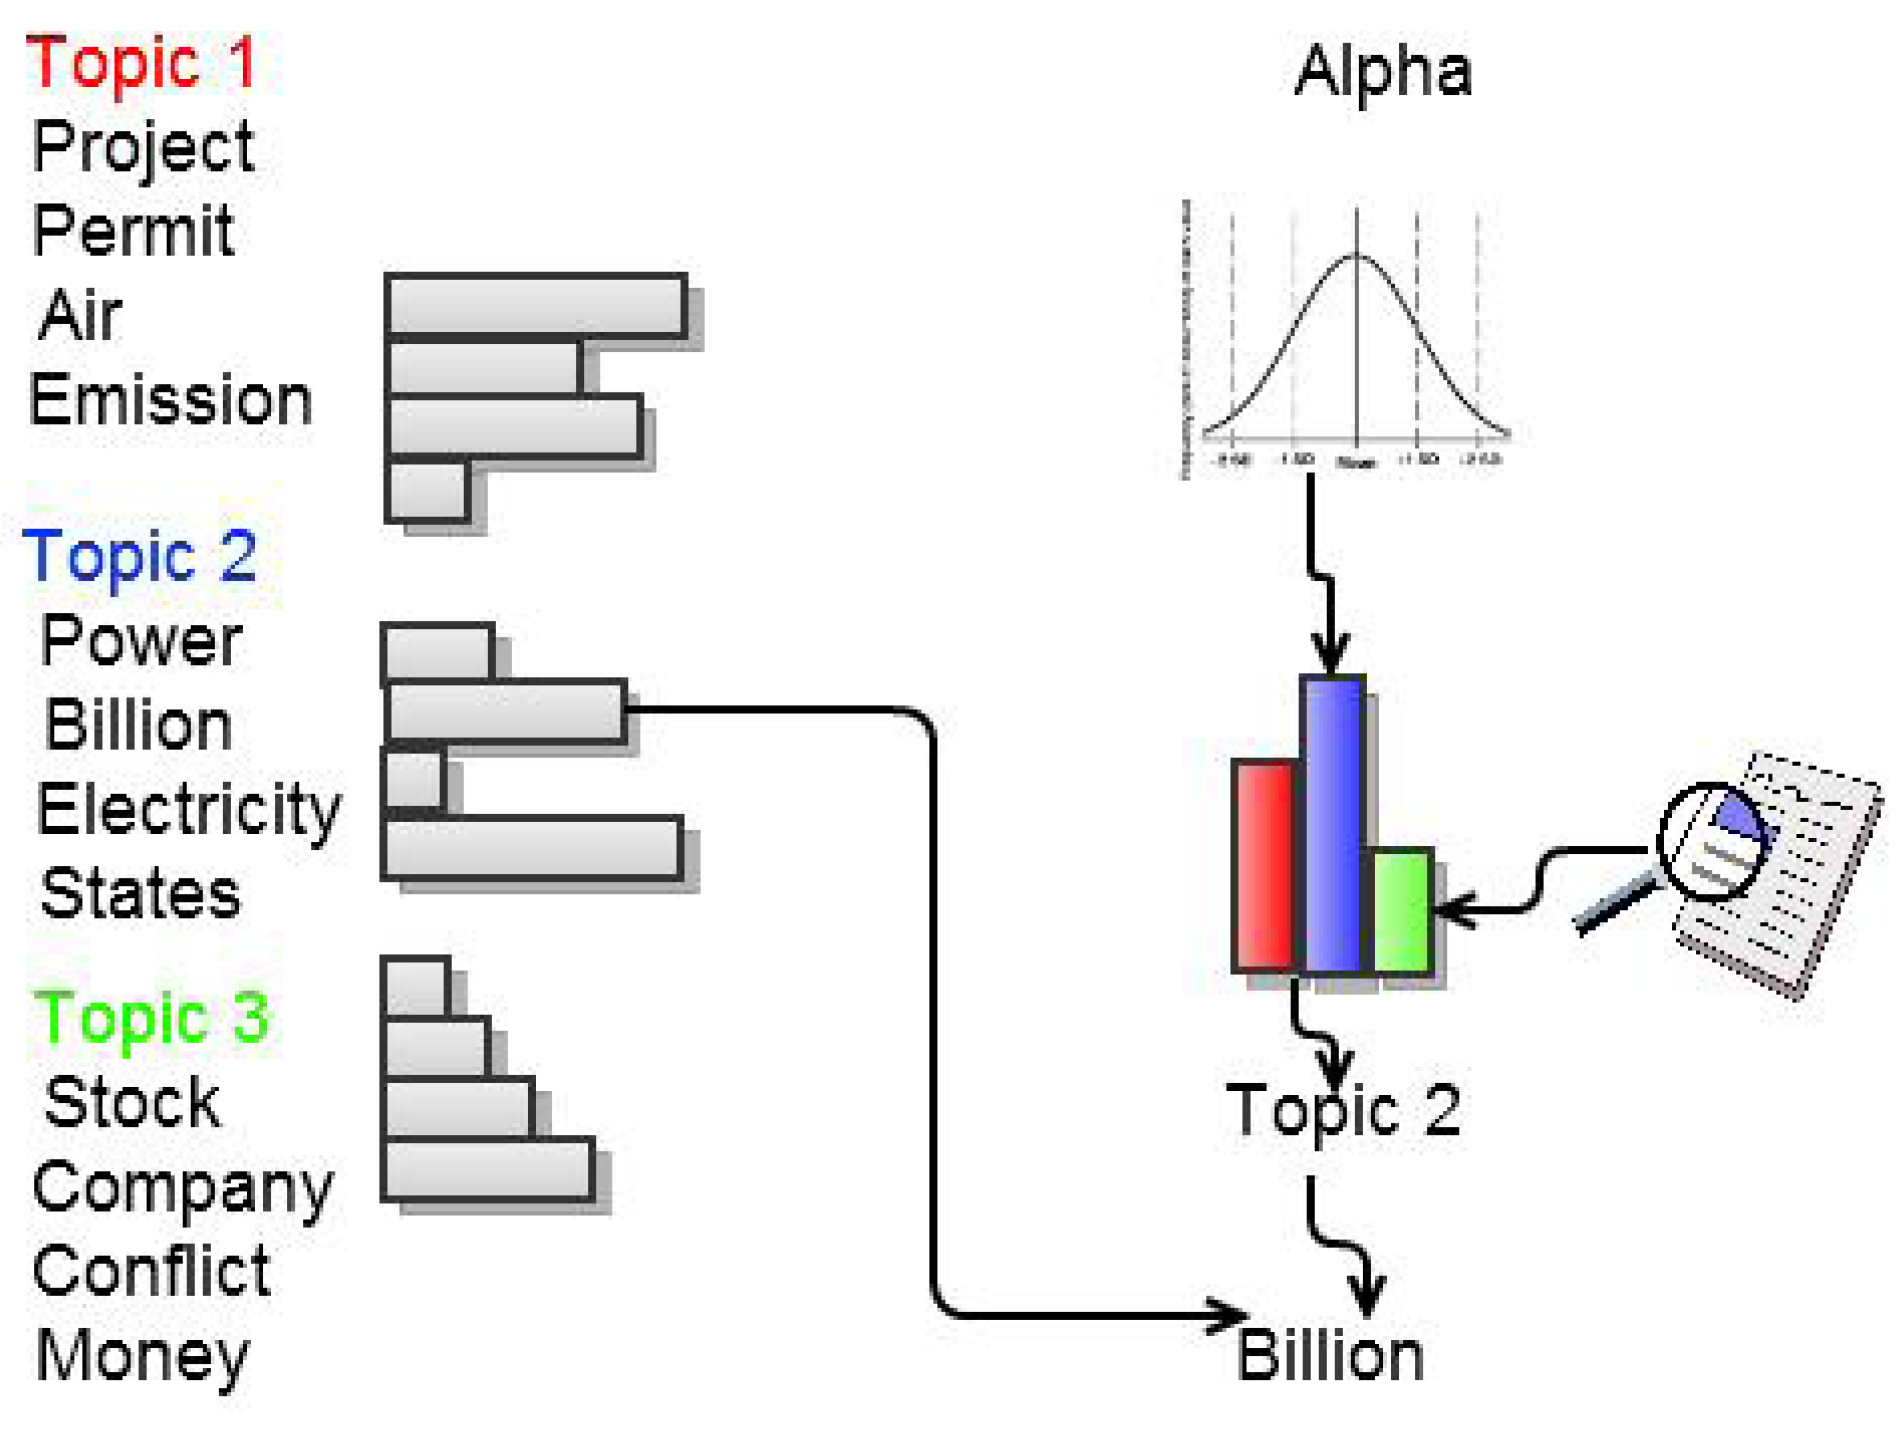
\includegraphics[scale=0.9]{../presentation_pics/lda_pres_pic1.png} \\
\vspace{0.4cm}
{\setstretch{1.0}\tiny Picture: Amogh Mahapatra, Nisheeth Srivastava and Jaideep Srivastava. Contextual Anomaly Detection in Text Data, \textit{Algorithms 2012}, pages 469-489, figure 3, 2012.\\}
\end{frame}

\begin{frame}
\frametitle{Underlying math (essentially)}
\begin{enumerate}
\item Use LDA to interpret the topic assignment as a problem in Bayesian inference
\item Variational inference:
\begin{itemize}
\item Using suitable family of approximations and metric, the problem is turned to optimization in a metric space
\item Doing suitable estimations and assumptions, problem is moved to $R^{n}$ and the target function (i.e. the metric) becomes tractable to compute
\end{itemize}
\end{enumerate}
\end{frame}

\begin{frame}
\frametitle{High-dimensional optimization}
\begin{tabular}{c c}
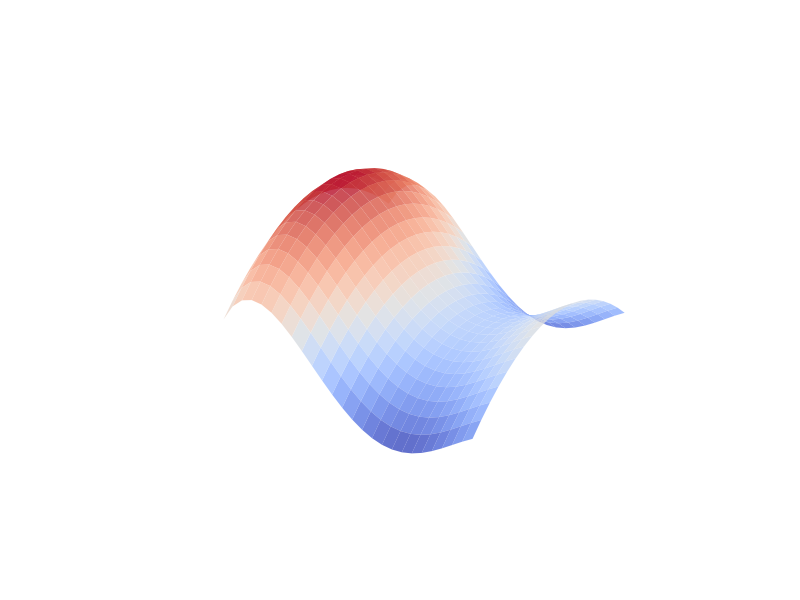
\includegraphics[trim= 30mm 30mm 30mm 30mm, scale = 0.4]{../presentation_pics/twodimensionalf.png} &
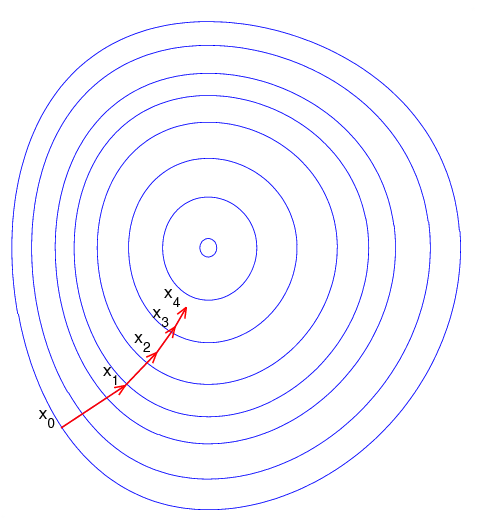
\includegraphics[scale=0.25]{../presentation_pics/Gradient_descent.png}
\end{tabular}
\end{frame}

\begin{frame}
\frametitle{Effect of dimension}
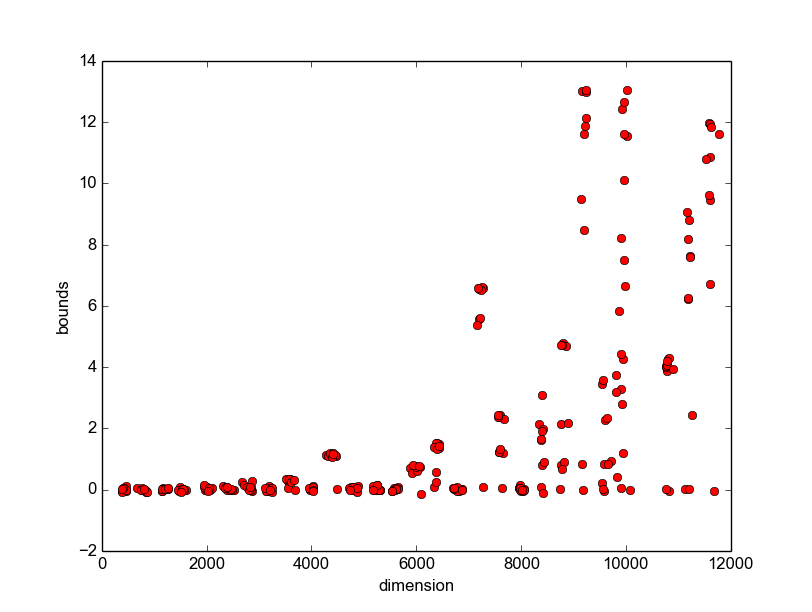
\includegraphics[scale=0.5]{../presentation_pics/FR_data_plain.png}
\end{frame}

\begin{frame}
\frametitle{Where do we end up?}
\begin{center}
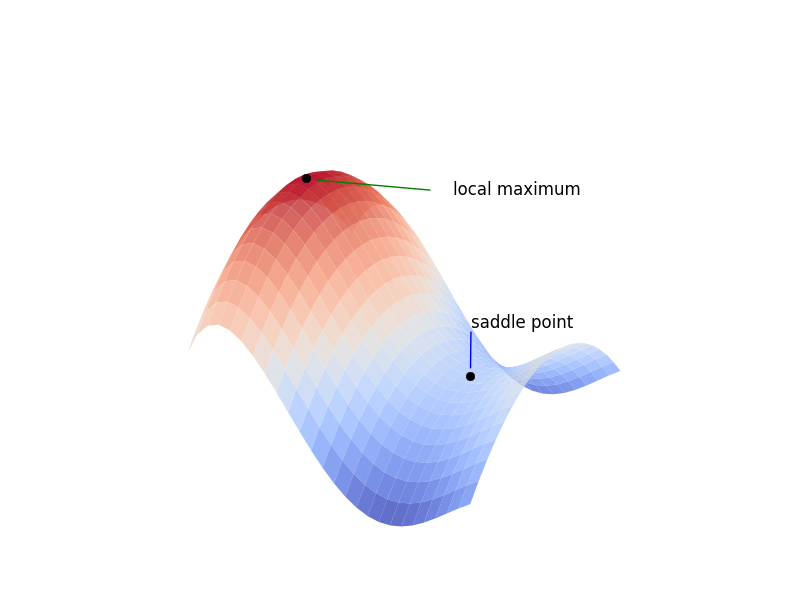
\includegraphics[trim=30mm 30mm 30mm 30mm,scale=0.3]{../presentation_pics/saddle_max_2.png}
\end{center}
\begin{tcolorbox}[title=Curse of dimensionality,colframe=green!40!black,colback=green!5]
``$\ldots$in high dimensions, the chance that all the directions around a critical point lead upward (positive curvature) is exponentially small$\ldots$'' (Dauphin et al. 2014$\footnotemark$)
\end{tcolorbox}

{\setstretch{1.0}\tiny \footnotemark[1]Yann N Dauphin, Razvan Pascanu, Caglar Gulcehre, Kyunghyun Cho, Surya Ganguli, and Yoshua Bengio. Identifying and attacking the saddle point problem in high-dimensional non-convex optimization. \textit{In Advances in Neural Information Processing Systems}, pages 2933-2941, 2014.\\}
\end{frame}

\begin{frame}
\frametitle{Effect of dimension, eigenvalues}
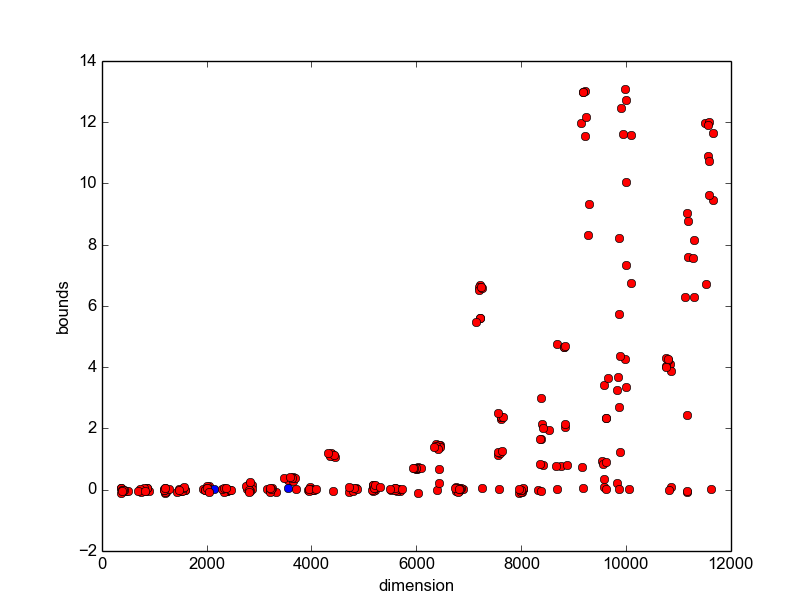
\includegraphics[scale=0.5]{../presentation_pics/FR_data_color.png}
\end{frame}

\begin{frame}
\frametitle{What next?}
\begin{itemize}
\item More info about the eigenvalues/local behaviour
\item Improving methods
\end{itemize}
\end{frame}

\begin{frame}
\frametitle{The main things}
To sum up:
\begin{itemize}
\item Turning topic assignment to high-dimensional optimization via
\begin{enumerate}
\item building a model
\item using variational ideas to deal with Bayesian inference
\end{enumerate}
\item In high-dimensional spaces, many simple ideas lose their edges
\end{itemize}
\end{frame}


\end{document}
